\section{Pedagogical Design}
\label{sec:pedagogy}

The design choices described in Sections~\ref{sec:architecture}
and~\ref{sec:circuit-solver} were each made with a specific misconception or missing
intuition in mind, in the spirit of Papert's constructionism~\cite{papert1980mindstorms}:
a learner builds a working artifact and inspects its behavior directly, rather than being
shown the artifact's behavior secondhand.

\textbf{Wiring as physical placement, not schematic capture.} A component's two leads are
specific block faces, and two blocks are electrically connected only if each presents a
conductive face to the other. This is closer to breadboarding than to drawing a schematic:
a player who wires a resistor and a capacitor in what they intend to be a series loop, but
leaves a gap, gets a demonstrably incomplete circuit (Section~\ref{sec:circuit-solver}'s
floating-node handling means this fails safely rather than crashing), the same way a real
breadboard with a missing jumper simply does not work, rather than a schematic tool
flagging an unconnected pin as an abstract error.

\textbf{An explicit ground reference.} ``Voltage is always relative to a chosen reference''
is a standard remark in an introductory course, but it is easy for a student to receive it
as trivia rather than as something with consequences, because a schematic tool typically
draws a ground symbol for you, already connected, wherever the exercise needs it. Requiring
a player to place a ground block and wire it in themselves before a wire's absolute voltage
reading becomes meaningful (Section~\ref{sec:circuit-solver}) makes the reference an object
the player is responsible for, not a background assumption.

\textbf{Sources that must be switched on.} Both voltage sources are wired to a redstone
input and remain electrically inert -- an open circuit, contributing nothing to the solved
system -- until that input is active. This mirrors an actual laboratory workflow (wire the
circuit completely, verify it, \emph{then} switch the bench supply on) and, as a side
effect, is what makes the topology bug described in Section~\ref{sec:topology-bug} safe to
discuss with students directly: a source that is allowed to inject current into a circuit
whose leads are still both landing on the same node is not a hypothetical hazard invented
for this mod, it is the textbook definition of shorting a source across itself, and the fix
is the same for a player's bad wiring as it was for the mod's own construction algorithm.

\textbf{An oscilloscope that can watch more than one thing at once.} A single-channel
readout answers ``what is this component doing'', but the more interesting classroom
question is usually comparative -- how does the capacitor's voltage lag the source
driving it, or how does a resistor's voltage track a memristor's drifting resistance --
which requires watching multiple points simultaneously and comparing their phase and shape
against each other, not just their instantaneous values in isolation. Figure~\ref{fig:scope}
shows the in-game oscilloscope pinned to three points in the same circuit at once (a
function generator, a capacitor, and a resistor), reproducing the same relative-phase
comparison a real bench oscilloscope's multiple channels are used for.

\begin{figure}[htbp]
\centering
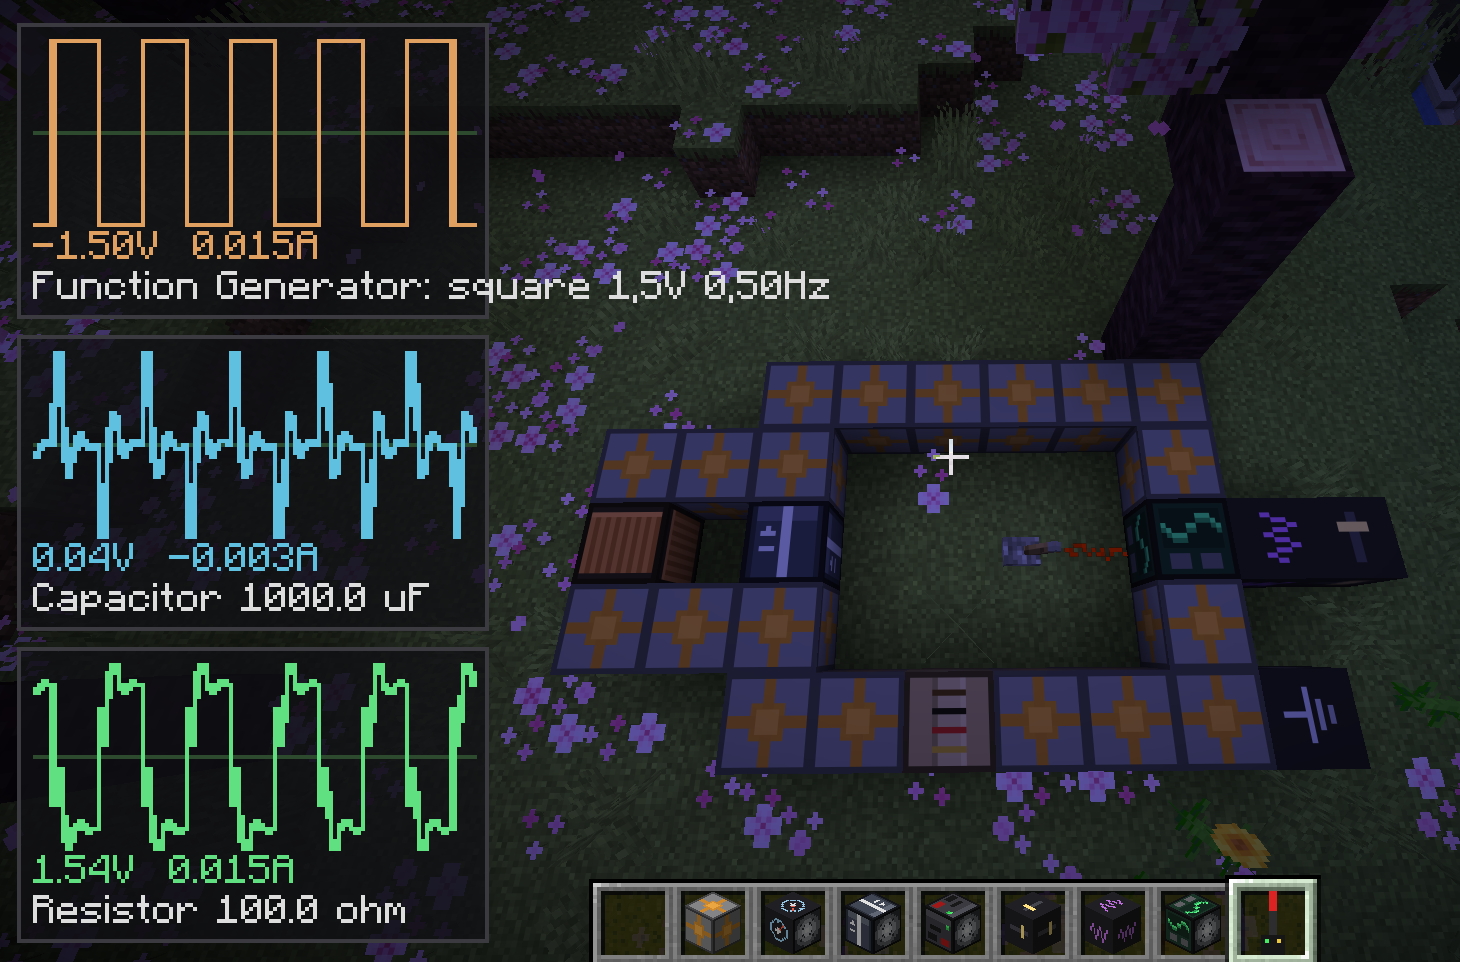
\includegraphics[width=0.48\textwidth]{figures/square_waveform.png}
\hfill
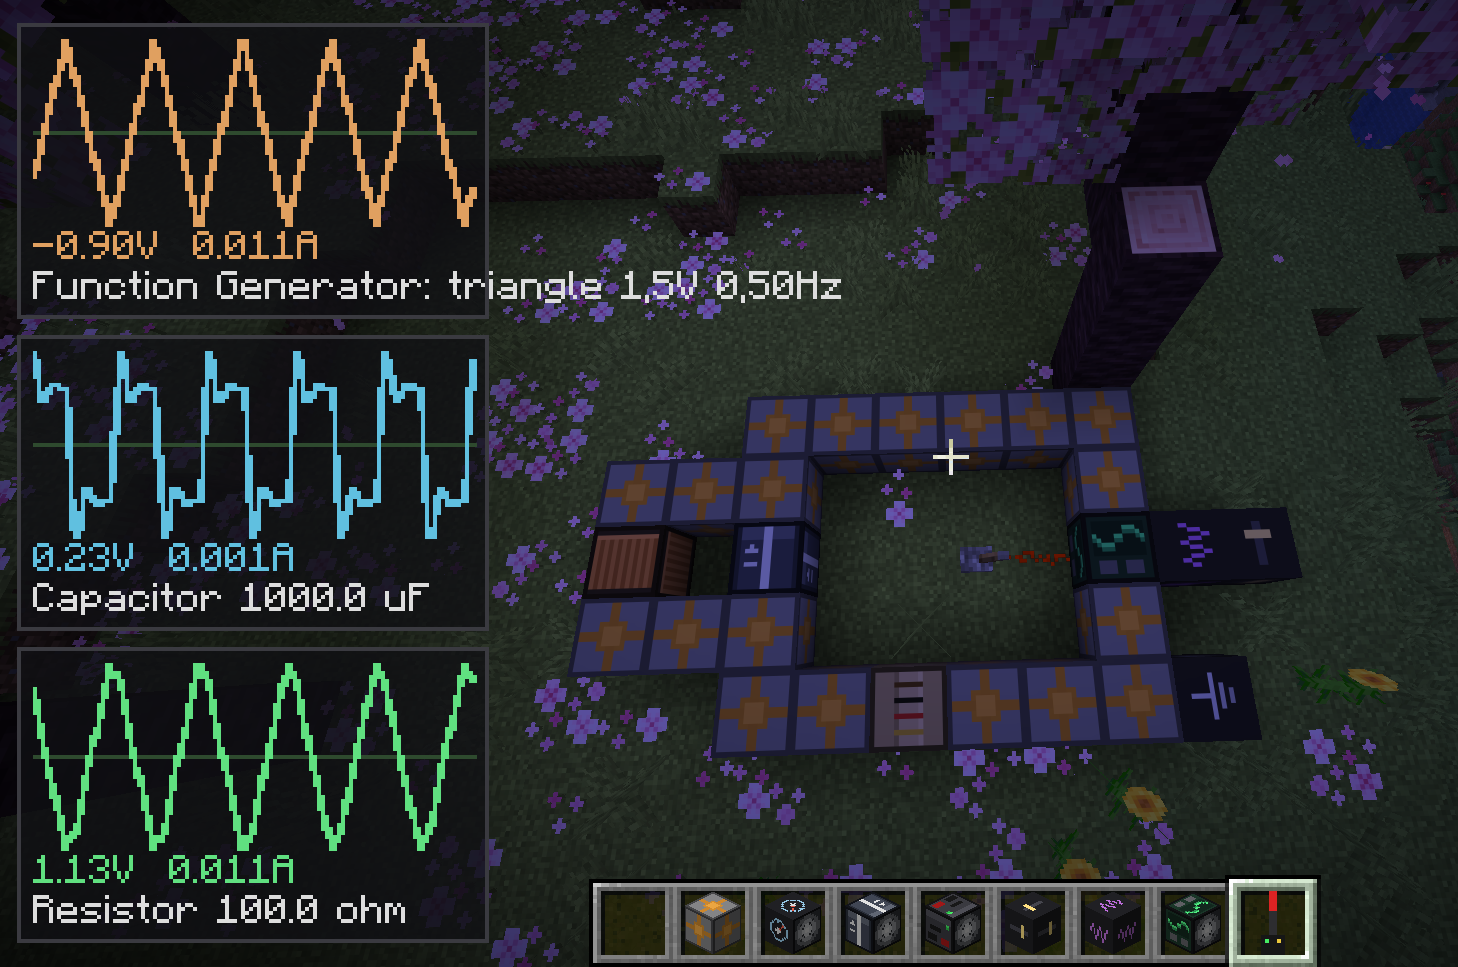
\includegraphics[width=0.48\textwidth]{figures/triangle_waveform.png}
\caption{The in-game multi-channel oscilloscope, pinned simultaneously to a function
generator (top trace), a capacitor (middle trace), and a resistor (bottom trace) in the same
circuit, driven by a square wave (left) and a triangle wave (right). Each trace is
independently auto-scaled and color-coded, with a live voltage/current readout and a summary
of that component's current state below its plot.}
\label{fig:scope}
\end{figure}
